\documentclass{beamer}
%\usetheme{Antibes}
\usetheme{Dresden}
%\usetheme{Frankfurt}
%\usetheme{Copenhagen}
%\usetheme{Darmstadt}
%\usecolortheme{dolphin}
\usepackage{cancel}
\usepackage{tikz}
%%%%%%%%%%%%%%%%%%%%%%%%%%%%%%%%%%%%%%%%%%%%%%%%%%%%%%%%
\usepackage{multicol}

\newtheorem{proposition}[theorem]{Proposition}
\newtheorem{remark}[theorem]{Remark}
\newtheorem*{remark*}{Remark}
\newtheorem{conjecture}[theorem]{Conjecture}
\newtheorem{claim}[theorem]{Claim}
\newtheorem*{claim*}{Claim}
\usepackage{xcolor}
\usepackage{longtable}
\usepackage{hyperref}
\newtheorem{openproblem}[theorem]{Open Problem}


\setbeamertemplate{blocks}[rounded][shadow=true]

\setbeamertemplate{theorems}[ams style]
\begin{document}
	\title[]{\textcolor{black}{\textbf{Classify Chest X-ray Images}}}
	
	\author[Yevgeniy Kostrov \hspace{1in} ekostrov@yahoo.com]
	{\textcolor{black}
	{\textbf{by Y.~Kostrov\inst}}}
	\date[April 14, 2019]

%
%	Title Page:
%	

%	{
%\usebackgroundtemplate{\includegraphics[height=\paperheight,width=\paperwidth]{london}}
%\frame{
%}
%}
	\begin{frame}	
			\maketitle
	\end{frame}
\begin{frame}{\contentsname}
	\begin{multicols}{2}
		\tableofcontents
	\end{multicols}
\end{frame}
%
%
%	
%
%
%}
\section{Overview}
\frame{
\frametitle{Overview }
\begin{center}
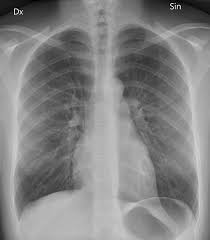
\includegraphics[width=1.8in]{first.png}\\
In this project, I create a model that will classify x-ray image of a chest as the one that has pneumonia or the one that doesn't have pneumonia
\end{center}
}
\section{Business Problem}
\frame{
\frametitle{Business Problem}
\begin{itemize}
	\item Pneumonia is a very dangerous diseases that is caused by a bacterial or viral infection of the lungs.
	\item The consequences of pneumonia could be catastrophic within a short period of time if not diagnosed quickly. 
	
	\item In this project I developed two models for the classification of chest X-ray images into NORMAL (no pneumonia) vs. PNEUMONIA(there is pneumonia in the lungs). 
\end{itemize}
}
\section{Data}
\frame{
\frametitle{Data Used in the Project}
\begin{itemize}
	\item Data for this project was downloaded from Mendeley Data: Large Dataset of Labeled Optical Coherence Tomography (OCT) and Chest X-Ray Images. 
	\vskip 0.2in
	\item Data consists of chest x-ray images of different size split into two directories for training and testing.
\end{itemize}
}
\frame{
	\frametitle{Number of Normal vs Pneumonia in Train Directory}
	\begin{center}
		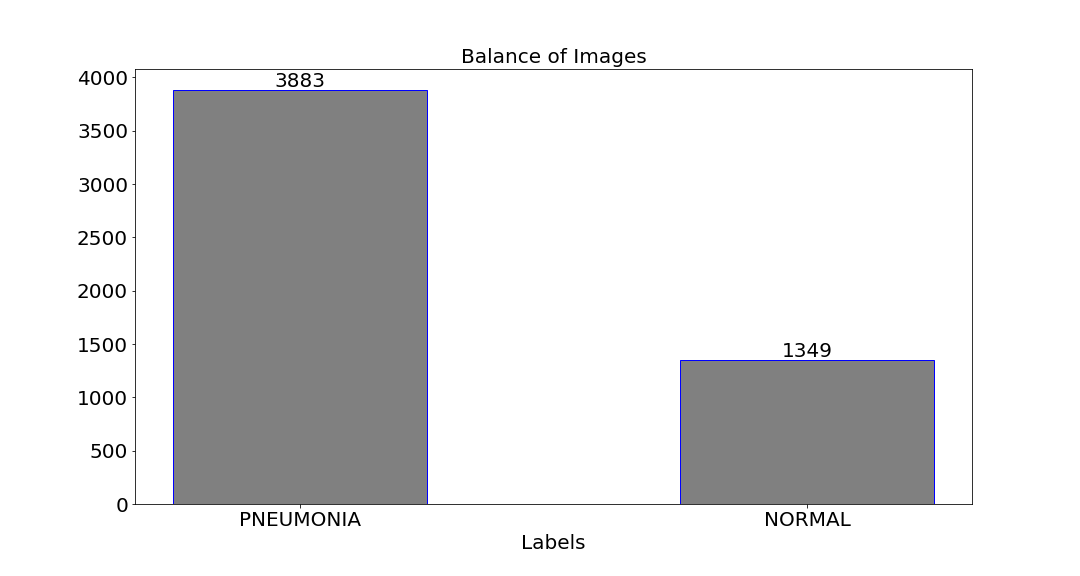
\includegraphics[width=4.5in]{second.png}
	\end{center}
}
\frame{
	\frametitle{Sample Images from Train Directory}
	\begin{center}
		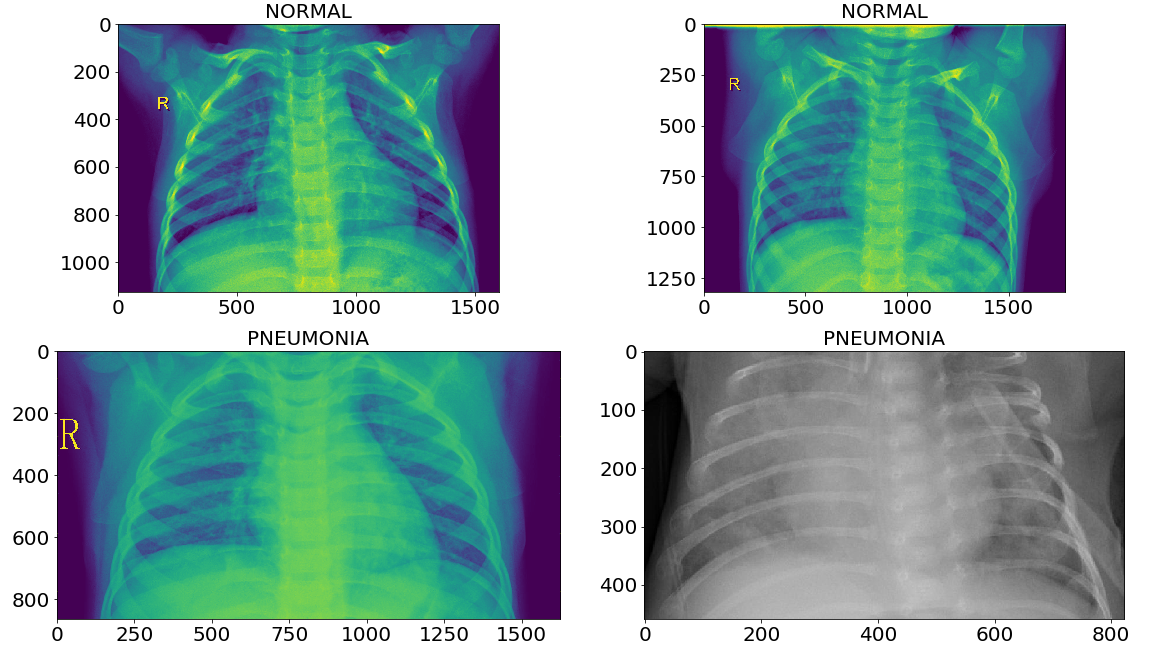
\includegraphics[width=4.5in]{third.png}
	\end{center}
}
\frame{
	\frametitle{Number of Normal vs Pneumonia in Test Directory}
	\begin{center}
		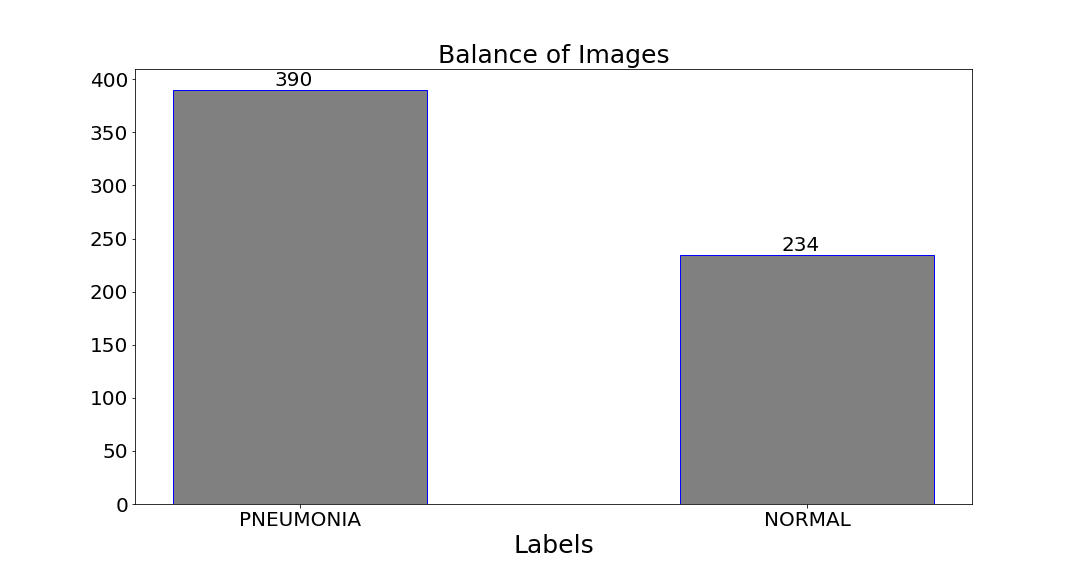
\includegraphics[width=4.5in]{fourth.png}
	\end{center}
}
\frame{
	\frametitle{Sample Images from Test Directory}
	\begin{center}
		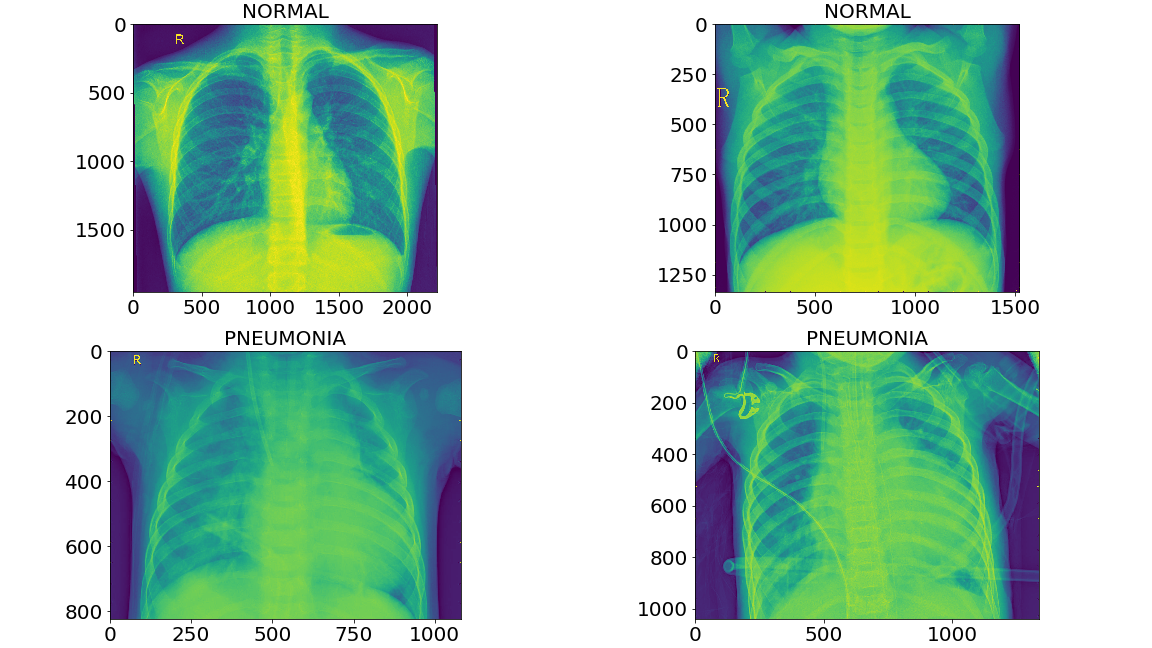
\includegraphics[width=4.5in]{fifth.png}
	\end{center}
}
\section{Modeling}
\frame{
\frametitle{Modeling: Creating  Models}
I have built the following two models 
\vskip 0.1in
\begin{itemize}
	\item Baseline Model from scratch
	\item Transfer Learning Model based on VGG19 trained on imagenet dataset.
\end{itemize}
I used recall as a primary metric and accuracy as a secondary metric for assessment of models.
}
\subsection{Metrics}
\frame{
\frametitle{Explanation of  Recall}
\begin{itemize}
\item Recall is defined as:
\[\small \text{Recall} = \frac{\text{True Positive}}{\text{True Positive + False Negative}} = \frac{\text{True Positive}}{\text{Total Actual Positive}}\] 
\end{itemize}
}
\frame{
	\frametitle{Explanation of Recall}
\begin{itemize}
	\item Recall calculates how many of the Actual Positives our model captures by marking it as Positive (True Positive). 
	\item Thus Recall is a better model metric  when there is a high cost associated with False Negative.
	\item In our case False Negative is predicting images as ”NORMAL” when in reality the image has the label ”PNEUMONIA”.
	\item	In this case pneumonia will not be diagnosed in the patient and consequnces might be drastic.
\end{itemize}
}
\frame{
\frametitle{Explanation of Recall}
\begin{itemize}
	\item For instance, in prediction of pneumonia. 
	\item If the case of pneumonia is predicted as normal(Predicted Negative), then the person who is sick will not be treated on time.
\end{itemize}
}
\frame{
\frametitle{Explanation of  Accuracy}
\begin{itemize}
	\item There is another metric we will use is called "accuracy".
	\item Accuracy is defined as:
	\[\small \text{Accuracy} = \frac{\text{Correct Predictions}}{\text{All Predictions}}\]
	\normalsize 
\end{itemize}
}
\frame{
	\frametitle{Explanation of Accuracy}
	\begin{itemize}
		\item Accuracy is the number of correctly predicted data points out of all the data points.
		\vskip 0.2in
		\item Often, accuracy is used along with recall.
	\end{itemize}
}

\section{Models' Performance}
\frame{
\frametitle{How Well Models Performed}
\begin{itemize}
	\item Baseline Model achieved 99\% on the recall metric and 87.5\% on accuracy score
	\vskip 0.3in
	\item Transfer Learning Model achieved 97.4\% on the  accuracy metric and it is, also, has accuracy at 97.6\%.
\end{itemize}
}
\section{Conclusions}
\frame{
\frametitle{Business Suggestion}
\begin{center}
	Based on my analysis, 
	\begin{itemize}
		\item I suggest to use  Transfer Learning model for the prediction of pneumonia in chest x-rays since it gets better balanced results between recall and accuracy metrics.	
	\end{itemize}
\end{center}
 
}
\frame{
\begin{center}
	\LARGE
	THE END \\
	THANK YOU!
\end{center}
}
\end{document}